\documentclass[a4]{article}
\usepackage{amssymb}
\usepackage{amsmath}
\usepackage{bm}
\usepackage{url}
\usepackage{graphicx}
\usepackage{mathtools}
\DeclareMathOperator*{\argmax}{argmax}
\DeclareMathOperator*{\argmin}{argmin}

\DeclarePairedDelimiter\ceil{\lceil}{\rceil}
\DeclarePairedDelimiter\floor{\lfloor}{\rfloor}

\newtheorem{defn}{Definition}

%opening
\title{DNN, CNN, RNN, LSTM, Attn, and Transformer}
\author{Shoichiro Yamanishi}



\begin{document}

\maketitle


\section{Introduction}

This document describes the following.
\begin{itemize}

\item DNN Backprop mechanism

\item CNN Forward propagation and Backprop in multi-channel 2-dimensional convolution kernel with step size $s$.

\item RNN Backprop

\item The reason of LSTM as a generalization of leaky units with learned parameters to cope with vanishing gradient problem.

\item Traditional Attention on top of bi-directional RNN

\item Transformer's multi-head attention part.

\end{itemize}

\section{Backprop : DNN}
The fully connected deep neural network is defined as follows.

\begin{equation}
\begin{aligned}
&\bm{x} : \text{sample input}\\
&\bm{y} : \text{sample output}\\
&W^{(i)} : \text{weights to be leaned}\\
&\bm{b}^{(i)} : \text{bias to be leaned}\\
&\bm{h}^{(0)} = \bm{x}\\
&\bm{a}^{(i)} = W^{(i)}\bm{h}^{(i-1)}+ \bm{b}^{(i)} : \text{activation at the i-th layer}\\
&\bm{h}^{(i)} = \bm{f}^{(i)}(\bm{a}^{(i)}) : \text{hidden variable at the i-th layer}\\
&\hat{\bm{y}} = \bm{h}^{(l)} : \text{output}\\
&J(\hat{\bm{y}}, \bm{y}) : \text{loss function}
\end{aligned}
\end{equation}
The back propagation (of the derivatives of the loss function) is derived as follows.
First, the top level:
\begin{equation}
\begin{aligned}
\frac{ \partial J }{ \partial \bm{h}^{(l)} } = \frac{ \partial J }{ \partial \hat{\bm{y}} }
\label{eq:dnn_g(0)}
\end{aligned}
\end{equation}
Equation \ref{eq:dnn_g(0)} corresponds to the first assignment to $\bm{g}$ in Algorithm 6.4 in pp 206 of
DL \cite{GoodBengCour16}.
\begin{equation}
\begin{aligned}
\frac{ \partial J }{ \partial \bm{a}^{(l)} } &= 
\frac{ \partial J }{ \partial \bm{h}^{(l)} }
\frac{ \partial \bm{h}^{(l)} }{ \partial \bm{a}^{(l)} } = 
\frac{ \partial J }{ \partial \hat{\bm{y}} }
\bm{f}^{(l)'}\\
\frac{ \partial J } { \partial W^{(l)} } &= 
\frac{ \partial J }{ \partial \hat{\bm{y}} }
\frac{ \partial \bm{h}^{(l)} }{ \partial \bm{a}^{(l)} }
\frac{ \partial \bm{a}^{(l)} }{ \partial W^{(l)} } = 
\frac{ \partial J }{ \partial \hat{\bm{y}} }
\bm{f}^{(l)'}
\bm{h}^{(l-1)}\\
\frac{ \partial J } { \partial \bm{b}^{(l)} } &= 
\frac{ \partial J }{ \partial \hat{\bm{y}} }
\frac{ \partial \bm{h}^{(l)} }{ \partial \bm{a}^{(l)} }
\frac{ \partial \bm{a}^{(l)} }{ \partial \bm{b}^{(l)} } = 
\frac{ \partial J }{ \partial \hat{\bm{y}} }
\bm{f}^{(l)'}
\end{aligned}
\end{equation}
Next, down to the bottom level.
\begin{equation}
\begin{aligned}
\frac{ \partial J } { \partial W^{(i)} } &= 
\frac{ \partial J } { \partial \bm{a}^{(i)} }
\frac{ \partial \bm{a}^{(i)} }{ \partial W^{(i)} } = 
\frac{ \partial J } { \partial \bm{a}^{(i)} }
\bm{h}^{(i-1)}\\
\frac{ \partial J } { \partial \bm{b}^{(i)} } &= 
\frac{ \partial J } { \partial \bm{a}^{(i)} }
\frac{ \partial \bm{a}^{(i)} }{ \partial \bm{b}^{(i)} } = 
\frac{ \partial J } { \partial \bm{a}^{(i)} }\\
\end{aligned}
\end{equation}
$\frac{ \partial J } { \partial \bm{a}^{(i)} }$, which corresponds to the second assignment to
$\bm{g}$ in Algorithm 6.4 in pp 206 of DL \cite{GoodBengCour16}, is recursively defined as follows.
\begin{equation}
\begin{aligned}
\frac{ \partial J } { \partial \bm{a}^{(i)} } &= 
\sum_{ \bm{a}^{(i+1)} }
\frac{ \partial J } { \partial \bm{a}^{(i+1)} }
\frac{ \partial \bm{a}^{(i+1)} }{ \partial \bm{a}^{(i)} }\\
&=\sum_{ \bm{a}^{(i+1)} }
\frac{ \partial J } { \partial \bm{a}^{(i+1)} }
\frac{ \partial \bm{a}^{(i+1)} }{ \partial \bm{h}^{(i)} }
\frac{ \partial \bm{h}^{(i)} }{ \partial \bm{a}^{(i)} }\\
&=\left(\sum_{ \bm{a}^{(i+1)} }
\frac{ \partial J } { \partial \bm{a}^{(i+1)} }
W^{(i)}\right)
\bm{f}^{(l)'}\label{eq:dnn_g(2)}\\
\end{aligned}
\end{equation}
where the facter inside the parenthesis corresponds to the third assignment to
$\bm{g}$ in Algorithm 6.4 in pp 206 of  DL \cite{GoodBengCour16}.

For general back propagation using the computational graph used by TensorFlow 
is presented in figure 6.11 of DL \cite{GoodBengCour16}.


\section{CNN}
Following the notational convention by DL \cite{GoodBengCour16}, one leyar of 2-dimentional
convolution layer from an input $V$ to its activation $Z$ with step $s$ is defined as follows.



\begin{equation}
\begin{aligned}
&V_{l,j,k}  \:\:\:\:\:-\:\:\:\:input\hspace{3.8em} l:\text{i-channel}\:\:\:\: j:\text{coord1}\:\:\:\:k:\text{coord2}\\
&K_{i,l,m,n} -\:\:\:\:conv\:kernel\:\:\:\: i:\text{o-channel} 
\:\:\:\: l:\text{i-channel}
\:\:\:\: m:\text{coord1}\:\:\:\:n:\text{coord1}\\
&Z_{i,j,k}  \:\:\:\:\:-\:\:\:\:activation\hspace{1.5em}
i:\text{o-channel}\:\:\:\: j:\text{coord1}\:\:\:\:k:\text{coord2}\\
&Z_{i,j,k} = c\left( K, V, s \right) = \sum_{l,m,n}\left[ V_{l, (j-1)s+m, (k-1)s+n} K_{i,l,m,n} \right]
\:\:\:-\:\:\:\text{forward propagation}
\end{aligned}
\end{equation}
$V$ can be an image with $l$ indexing over the RGBA channel, and $j,k$ over the xy-coordinates.
$s$ is the step size over $V$.
Please see figure \ref{fig:cnn} and  \ref{fig:cnn_G}.

\begin{figure}[!htb]
\centering
\includegraphics[width=8cm]{cnn.png}
\caption{CNN Architecture}
\label{fig:cnn}
\end{figure}


\begin{figure}[!htb]
\centering
\includegraphics[width=8cm]{cnn_G.png}
\caption{Forward Propagation with Convolution}
\label{fig:cnn_G}
\end{figure}

\subsection{Backprop}
Assume the backprop is available up to $Z$ as in:
\begin{equation}
\begin{aligned}
G_{i,j,k} = \frac{\partial}{Z_{i,j,k}}J(\hat{\bm{y}}, \bm{y})
\end{aligned}
\end{equation}
We want to find $\frac{\partial}{K_{i,l,m,n}}J(\hat{\bm{y}}, \bm{y})$ for parameter update, and
 $\frac{\partial}{V_{l,j, k}}J(\hat{\bm{y}}, \bm{y})$ to back propagate the derivattive down
the network.

\begin{equation}
\begin{aligned}
g(G,V,s)_{i,l,m,n} &= \frac{\partial}{\partial K_{i,l,m,n}}J(\hat{\bm{y}}, \bm{y})\\
&= \sum \frac{\partial J}{\partial Z}\frac{\partial Z}{\partial K}\\
&= \sum_{j,k}G_{i, j, k}V_{l, (j-1)s+m, (k-1)s+n }
\end{aligned}
\end{equation}


\begin{figure}[!htb]
\centering
\includegraphics[width=8cm]{cnn_bp_K.png}
\caption{Backward Propagation to $g(G,V,s)_{i,l,m,n} = \frac{\partial}{\partial K_{i,l,m,n}}J(\hat{\bm{y}}, \bm{y})$}
\label{fig:cnn_bk_K}
\end{figure}


\begin{equation}
\begin{aligned}
h(K,G,s)_{l,j^V,k^V} &= \frac{\partial}{\partial V_{l,j^V,k^V}}J(\hat{\bm{y}}, \bm{y})\\
&= \sum \frac{\partial J}{\partial Z}\frac{\partial Z}{\partial V}\\
&= \sum_{j^Z,m}^{s.t.(j^Z-1)s+m=j^V}
   \sum_{k^Z,n}^{s.t.(k^Z-1)s+n=k^V}
   \sum_{i}
   K_{i, l, m, n}G_{i, j^Z, k^Z}
\end{aligned}
\end{equation}


\begin{figure}[!htb]
\centering
\includegraphics[width=8cm]{cnn_bp_h.png}
\caption{Backward Propagation to  $h(K,G,s)_{l,j^V,k^V} = \frac{\partial}{\partial V_{l,j^V,k^V}}J(\hat{\bm{y}}, \bm{y})$}
\label{fig:cnn_bk_h}
\end{figure}


\section{RNN}
Here I explain a simple case where the hidden layer uses $tanh$ and the final layer $softmax$.

\begin{equation}
\begin{aligned}
\bm{a}^{(t)} &= \bm{b} + W\bm{h}^{(t-1)} + U\bm{x}^{(t)}\\
\bm{h}^{(t)} &= tanh(\bm{a}^{(t)})\\
\bm{o}^{(t)} &= \bm{c}+ V\bm{h}^{(t)}\\
\hat{\bm{y}}^{(t)} &= softmax(\bm{o}^{(t)})\\
\end{aligned}
\end{equation}


\begin{figure}[!htb]
\centering
\includegraphics[width=8cm]{rnn.png}
\caption{Typical RNN}
\label{fig:rnn}
\end{figure}

\subsection{Backprop}

\begin{equation}
\begin{aligned}
\left[\frac{\partial J}{\partial \bm{o}^{(t)}}\right]_i 
&=
\left[\frac{\partial softmax(\bm{o}^{(t)})}{\partial \bm{o}^{(t)}}\right]_i\\
 &= \left(
\delta_{i,j}^{(t)} - \frac{\exp(o_i)}{\sum_k \exp(o_k)}
\right) \:\:\: \text{where}\:\:\hat{y}_j = 1\\
\\
\frac{\partial J}{\partial V} &= \sum_{t} \frac{\partial J}{\partial \bm{o}^{(t)}}
\frac{\partial \bm{o}^{(t)}}{\partial V}\\
&= \sum_{t} \frac{\partial J}{\partial \bm{o}^{(t)}}
\bm{h}^{(t)}\\
\\
\frac{\partial J}{\partial \bm{c}} &= \sum_{t} \frac{\partial J}{\partial \bm{o}^{(t)}}
\frac{\partial \bm{o}^{(t)}}{\partial \bm{c}}\\
&= \sum_{t} \frac{\partial J}{\partial \bm{o}^{(t)}}\\
\\
\frac{\partial J}{\partial \bm{h}^{(t)}} &=
\frac{\partial J}{\partial \bm{h}^{(t+1)}}
\frac{\partial \bm{h}^{(t+1)}}{\partial \bm{h}^{(t)}} +
\frac{\partial J}{\partial \bm{o}^{(t)}}
\frac{\partial \bm{o}^{(t)}}{\partial \bm{h}^{(t)}}\\
&=
\frac{\partial J}{\partial \bm{h}^{(t+1)}}
\frac{\partial \bm{h}^{(t+1)}}{\partial \bm{a}^{(t+1)}}
\frac{\partial \bm{a}^{(t+1)}}{\partial \bm{h}^{(t)}} +
\frac{\partial J}{\partial \bm{o}^{(t)}}
\frac{\partial \bm{o}^{(t)}}{\partial \bm{h}^{(t)}}\\
&=
\frac{\partial J}{\partial \bm{h}^{(t+1)}}
diag\left(\frac{\partial \tanh(\bm{a}^{(t+1)})}{\partial \bm{a}^{(t+1)}}\right)W +
\frac{\partial J}{\partial \bm{o}^{(t)}}V\\
\end{aligned}
\end{equation}

\begin{equation}
\begin{aligned}
\frac{\partial J}{\partial \bm{a}^{(t)}} &=
\frac{\partial J}{\partial \bm{h}^{(t)}}
\frac{\partial \bm{h}^{(t)}}{\partial \bm{a}^{(t)}}\\
&=
\frac{\partial J}{\partial \bm{h}^{(t)}}
diag\left(\frac{\partial \tanh(\bm{a}^{(t)})}{\partial \bm{a}^{(t)}}\right)\\
\\
\frac{\partial J}{\partial W} &=
\sum_{t}
\frac{\partial J}{\partial \bm{h}^{(t)}}
\frac{\partial \bm{h}^{(t)}}{\partial W}\\
&=
\sum_{t}
\frac{\partial J}{\partial \bm{h}^{(t)}}
\frac{\partial \bm{h}^{(t)}}{\partial \bm{a}^{(t)}}
\frac{\partial \bm{a}^{(t)}}{\partial W}\\
&=
\sum_{t}
\frac{\partial J}{\partial \bm{h}^{(t)}}
diag\left(\frac{\partial \tanh(\bm{a}^{(t)})}{\partial \bm{a}^{(t)}}\right)
\bm{h}^{(t-1)}
\\
\frac{\partial J}{\partial U} &=
\sum_{t}
\frac{\partial J}{\partial \bm{h}^{(t)}}
\frac{\partial \bm{h}^{(t)}}{\partial U}\\
&=
\sum_{t}
\frac{\partial J}{\partial \bm{h}^{(t)}}
\frac{\partial \bm{h}^{(t)}}{\partial \bm{a}^{(t)}}
\frac{\partial \bm{a}^{(t)}}{\partial U}\\
&=
\sum_{t}
\frac{\partial J}{\partial \bm{h}^{(t)}}
diag\left(\frac{\partial \tanh(\bm{a}^{(t)})}{\partial \bm{a}^{(t)}}\right)
\bm{x}^{(t)}
\\
\frac{\partial J}{\partial \bm{b}} &=
\sum_{t}
\frac{\partial J}{\partial \bm{h}^{(t)}}
\frac{\partial \bm{h}^{(t)}}{\partial \bm{b}}\\
&=
\sum_{t}
\frac{\partial J}{\partial \bm{h}^{(t)}}
\frac{\partial \bm{h}^{(t)}}{\partial \bm{a}^{(t)}}
\frac{\partial \bm{a}^{(t)}}{\partial \bm{b}}\\
&=
\sum_{t}
\frac{\partial J}{\partial \bm{h}^{(t)}}
diag\left(\frac{\partial \tanh(\bm{a}^{(t)})}{\partial \bm{a}^{(t)}}\right)
\end{aligned}
\end{equation}


\section{LSTM}
For the explanation of LSTM, please see colah's blog \cite{colah}. That is probably the best explanation
available publicly.
This section explains 'why' part as a generalization of \emph{leaky units}\cite{mosar}\cite{elhihi_bengio}.

The original problem with RNN is called \emph{vanishing gradient} problem where the gradient vanishes or
diverges during the backpropagation cycle depicted in figure \ref{fig:rnn2}.
This is similar to repeated multiplication of square matrix, which diverges or converges along eigen vectors.


\begin{figure}[!htb]
\centering
\includegraphics[width=8cm]{rnn2.png}
\caption{Gradient along the Back-propagation may Vanish or Diverge in RNN}
\label{fig:rnn2}
\end{figure}


This is mitigated by leaky units as in figure \ref{fig:leaky_unit}. Pelase note that the recursion does not involve
multiplication, but this is a kind of moving average.
The leaky units use a fixed parameter $\alpha$. 

\begin{figure}[!htb]
\centering
\includegraphics[width=8cm]{leaky_unit.png}
\caption{Recurrence with Leaky Units}
\label{fig:leaky_unit}
\end{figure}

LSTM generalizes it as a learned parameter as in figure \ref{fig:lstm}.

\begin{figure}[!htb]
\centering
\includegraphics[width=12cm]{lstm.png}
\caption{LSTM}
\label{fig:lstm}
\end{figure}

The main part of LSTM is formulated as follows.
\begin{equation}
\begin{aligned}
\bm{c}^{(t)} &= \alpha_i \tanh\left(W_c
\begin{bmatrix}
\bm{h}^{(t-1)}\\
\bm{x}^{(t)}\\
\end{bmatrix}
 + \bm{b}_c
\right)
+ \alpha_f \bm{c}^{(t-1)}\label{eq:lstm1}\\
\end{aligned}
\end{equation}
\begin{equation}
\begin{aligned}
\hspace{-10em}\bm{h}^{(t)} = \alpha_o \tanh(\bm{c}^{(t)})\label{eq:lstm2}\\
\end{aligned}
\end{equation}

The first term in equation \ref{eq:lstm1} represents the traditional RNN part, and
the second term is for the additive cell memory part, which is analogous to leaky unit.
Those terms are controlled by the following gates.
I think the $\tanh$ in equation  \ref{eq:lstm2} works as a layer-wise normalization.

\begin{equation}
\begin{aligned}
\alpha_i &= \sigma\left(W_i
\begin{bmatrix}
\bm{h}^{(t-1)}\\
\bm{x}^{(t)}\\
\end{bmatrix}
 + \bm{b}_i
\right)\\
\alpha_f &= \sigma\left(W_f
\begin{bmatrix}
\bm{h}^{(t-1)}\\
\bm{x}^{(t)}\\
\end{bmatrix}
 + \bm{b}_f
\right)\\
\alpha_o &= \sigma\left(W_o
\begin{bmatrix}
\bm{h}^{(t-1)}\\
\bm{x}^{(t)}\\
\end{bmatrix}
 + \bm{b}_o
\right)
\end{aligned}
\end{equation}



\section{Attention}
Attention is a mechanism to handle variable length input and also variable length output for 
sequence-to-sequence learning.
It is traditionally combined with bi-directional RNN.
Plase see figure \ref{fig:attention}.

\begin{figure}[!htb]
\centering
\includegraphics[width=10cm]{attention.png}
\caption{Attention Mechanism over Bi-Directional RNNs}
\label{fig:attention}
\end{figure}

The blue parts indicate the attention mechanism.
The lower part with $\bm{x}_i$, $\bm{h}_{f_i}$, and $\bm{h}_{b_i}$ is the standard
bi-directional RNN of length $Ni$. We combine both the forward and the backward vector into one as follows.
\begin{equation}
\begin{aligned}
\bm{h}_i &= 
\begin{bmatrix}
\bm{h}_{f_i}\\
\bm{h}_{b_i}\\
\end{bmatrix}
\end{aligned}
\end{equation}
The output $\bm{y}_j$ is generated from its corresponding hidden variable $\bm{s}_j$.
$\bm{s}_j$ is generated from both $\bm{s}_{j-1}$ and a variable called context vector $\bm{c}_{j}$
An example is as follows, but this is not an essential part of the attention machanism. Any other
generation will be possible.

\begin{equation}
\begin{aligned}
\bm{y}_j &= W_y\bm{s}_j\\
\bm{s}_j &= sigmoid\left( W_s 
\begin{bmatrix}
\bm{s}_{j_i}\\
\bm{c}_{j}\\
\end{bmatrix}
\right)\:\:\:\:\text{element-wise}\\
\end{aligned}
\end{equation}

The context vector $\bm{c}_{j}$ is a weighted sum of the bi-directional hidden variables $\bm{h}_i$,
i.e., attention into $\bm{h}_i$.

\begin{equation}
\begin{aligned}
\bm{c}_j &= \sum_{i}^{Ni}\alpha_{i,j}\bm{h}_i\\
\end{aligned}
\end{equation}

The weights $\alpha_{i,j}$ are calculated from $\bm{s}_{j-1}$ and all the $\bm{h}_i$s as follows.
First, we calculate a similarity between $\bm{s}_{j-1}$ and each $\bm{h}_i$. Usually one of the
following is used.

\begin{equation}
\begin{aligned}
score_1\left( \bm{s}_{j-1}, \bm{h}_i\right) &= cosine\left(\bm{s}_{j-1}, \bm{h}_i \right)\\
\\
score_2\left( \bm{s}_{j-1}, \bm{h}_i\right) &= \bm{v}_t^T \tanh\left(W_t 
\begin{bmatrix}
\bm{s}_{j-1}\\
\bm{h}_{i}\\
\end{bmatrix}
\right)\\
\\
score_3\left( \bm{s}_{j-1}, \bm{h}_i\right) &= \frac{1}{\sqrt{d}}\bm{s}_{j-1}^T\bm{h}_i
\:\:\:\:d\:\:\text{is the length of}\:\:\bm{h}_i\\
\end{aligned}
\end{equation}

Then weights $\alpha_{i,j}$ is calculated as follows.

\begin{equation}
\begin{aligned}
\begin{bmatrix}
\alpha_{1,j}\\
\alpha_{2,j}\\
\cdots\\
\alpha_{Ni,j}\\
\end{bmatrix}
= softmax\Big(
\begin{bmatrix}
score_x\left( \bm{s}_{j-1}, \bm{h}_1\right)\\
score_x\left( \bm{s}_{j-1}, \bm{h}_2\right)\\
\cdots\\
score_x\left( \bm{s}_{j-1}, \bm{h}_{Ni}\right)\\
\end{bmatrix}\Big)
\end{aligned}
\end{equation}

Here $W_y$, $W_s$, $\bm{v}_s$, and $W_t$ are parameters to be learned.

\section{Transformer}
Transformer is an encoder-decoder mechanism to handle variable length input and output.
This section explains Transformer by constructing it from the bottmom up to the top.

The bottom part is the attention mechanism, which works as a soft version of key-value query.
The input to the query is a vector $\bm{q}$ of size $dim_i$. The output is a vector $\bm{r}$ of
size $dim_o$. Assume the number of the key-value pairs is $L$. The key-value pairs are
represented by two matrices $K \in \mathcal{R}^{L \times dim_i} = 
\begin{bmatrix}
\bm{k}_1\\
\bm{k}_2\\
\cdots
\bm{k}_{dim_i}\\
\end{bmatrix}
$ and
$ \in \mathcal{R}^{L \times dim_o} =
\begin{bmatrix}
\bm{v}_1\\
\bm{v}_2\\
\cdots
\bm{v}_{dim_o}\\
\end{bmatrix}
$. For given $\bm{q}$ a suitable key $\bm{k}_i$ is chosen based on the similarity, and the 
corresponding $\bm{v}_i$ is returned as $\bm{r}$
This is \emph{soft} in the sense that the key's similarity is measured by the scaled dot product,
and the value is chosen by $softmax$. Please see figure \ref{fig:transformer1}


\begin{figure}[!htb]
\centering
\includegraphics[width=12cm]{transformer1.png}
\caption{Single Soft Query for K-V Pairs}
\label{fig:transformer1}
\end{figure}


\begin{figure}[!htb]
\centering
\includegraphics[width=12cm]{transformer2.png}
\caption{From a Single Input to Multi-Head Attention}
\label{fig:transformer2}
\end{figure}

Next, we elaborate the single query into the multi-head attention used in Transformer.
See figure \ref{fig:transformer2}. (a) corresponds to figure \ref{fig:transformer1}.
(b) expands the single query to a sequence $Q$ of length $N_{input}$. (c) introduces linear
transformations $W_Q$, $W_K$, and $W_V$ to $Q$, $K$, and $V$ respectively. It usually reduces
dimensionality. (d) represents the multi-head attention in which there are 8 parallel queries,
each with its own linear transformations. The results are simply concatenated element-wise.
For Transformer, the input is a sequence of a word embedding with relative positional embedding
such as $cos(\theta_{word\_pos}), sin(\theta_{word\_pos})$. Above concatenated $R$ sits 
leyer-wise normalization, element-wise fully connected NN, and layer-wise normalization with
some skip connections, which can be seen in the original paper \cite{transformer}.

\bibliography{dnn_cnn_rnn_lstm_attention.bib}{}
\bibliographystyle{plain}


\end{document}

